\section{Mind Maps}
\label{research:MindMaps}

My Goals:
\begin{itemize}
    \item I am trying to find a system for visually displaying information to the user in a manner that primarily boosts note searchability but is also visually appealing as to be interesting
    \item The system should be automatically generated by the computer so that the user doesn’t have to spend their time making the notes arrange nicely, instead they can focus on the note content itself
    \item The system should nicely integrate in a visual way with my searching tools so that the user can choose to click around and browse the structure or search for key terms
\end{itemize}


This initial image below acts as some inspiration for me as ideas are visually linked to each other and a path can be created through following the hierarchy of elements. Whilst I have previously avoided mind maps (the limiting nature of physically drawing elements out and the difficulty in later reorganizing my formatting frustrated me) a powerful digital version of this would meet all my criteria.

\begin{figure}[H]
    \centering
    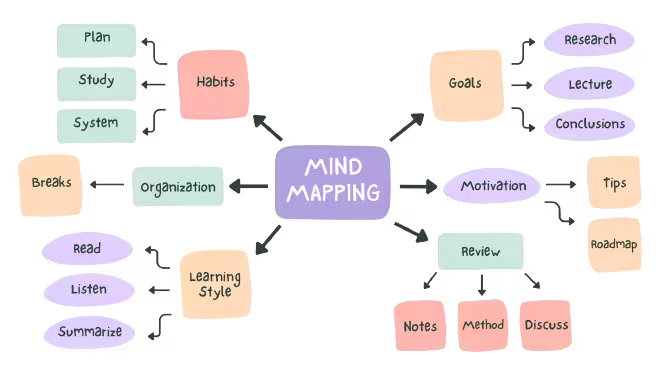
\includegraphics[width=0.8\textwidth]{Research/6_MindMaps/media/InspirationMindMap.png}
    \caption{Example of a mind map}
\end{figure}

Before researching the technical aspects of a system such as this I had a look at how mind maps(and alternative note methods) work alongside human learning, as without this having a clear link this was a pointless path to explore

\subsection*{Industry use}
\begin{figure}[H]
    \centering
    
\includegraphics[width=0.8\textwidth]{Research/6_MindMaps/media/artwork.png}
    \caption{Creative Mindmap Visualisations}

\end{figure}
Images like these are very common in the creative industry, they are used to visually represent ideas and concepts in a way that is easy to understand however they are not neccisarily as easy to navigate or to search for a specfici item.

\begin{figure}[H]
    \centering
    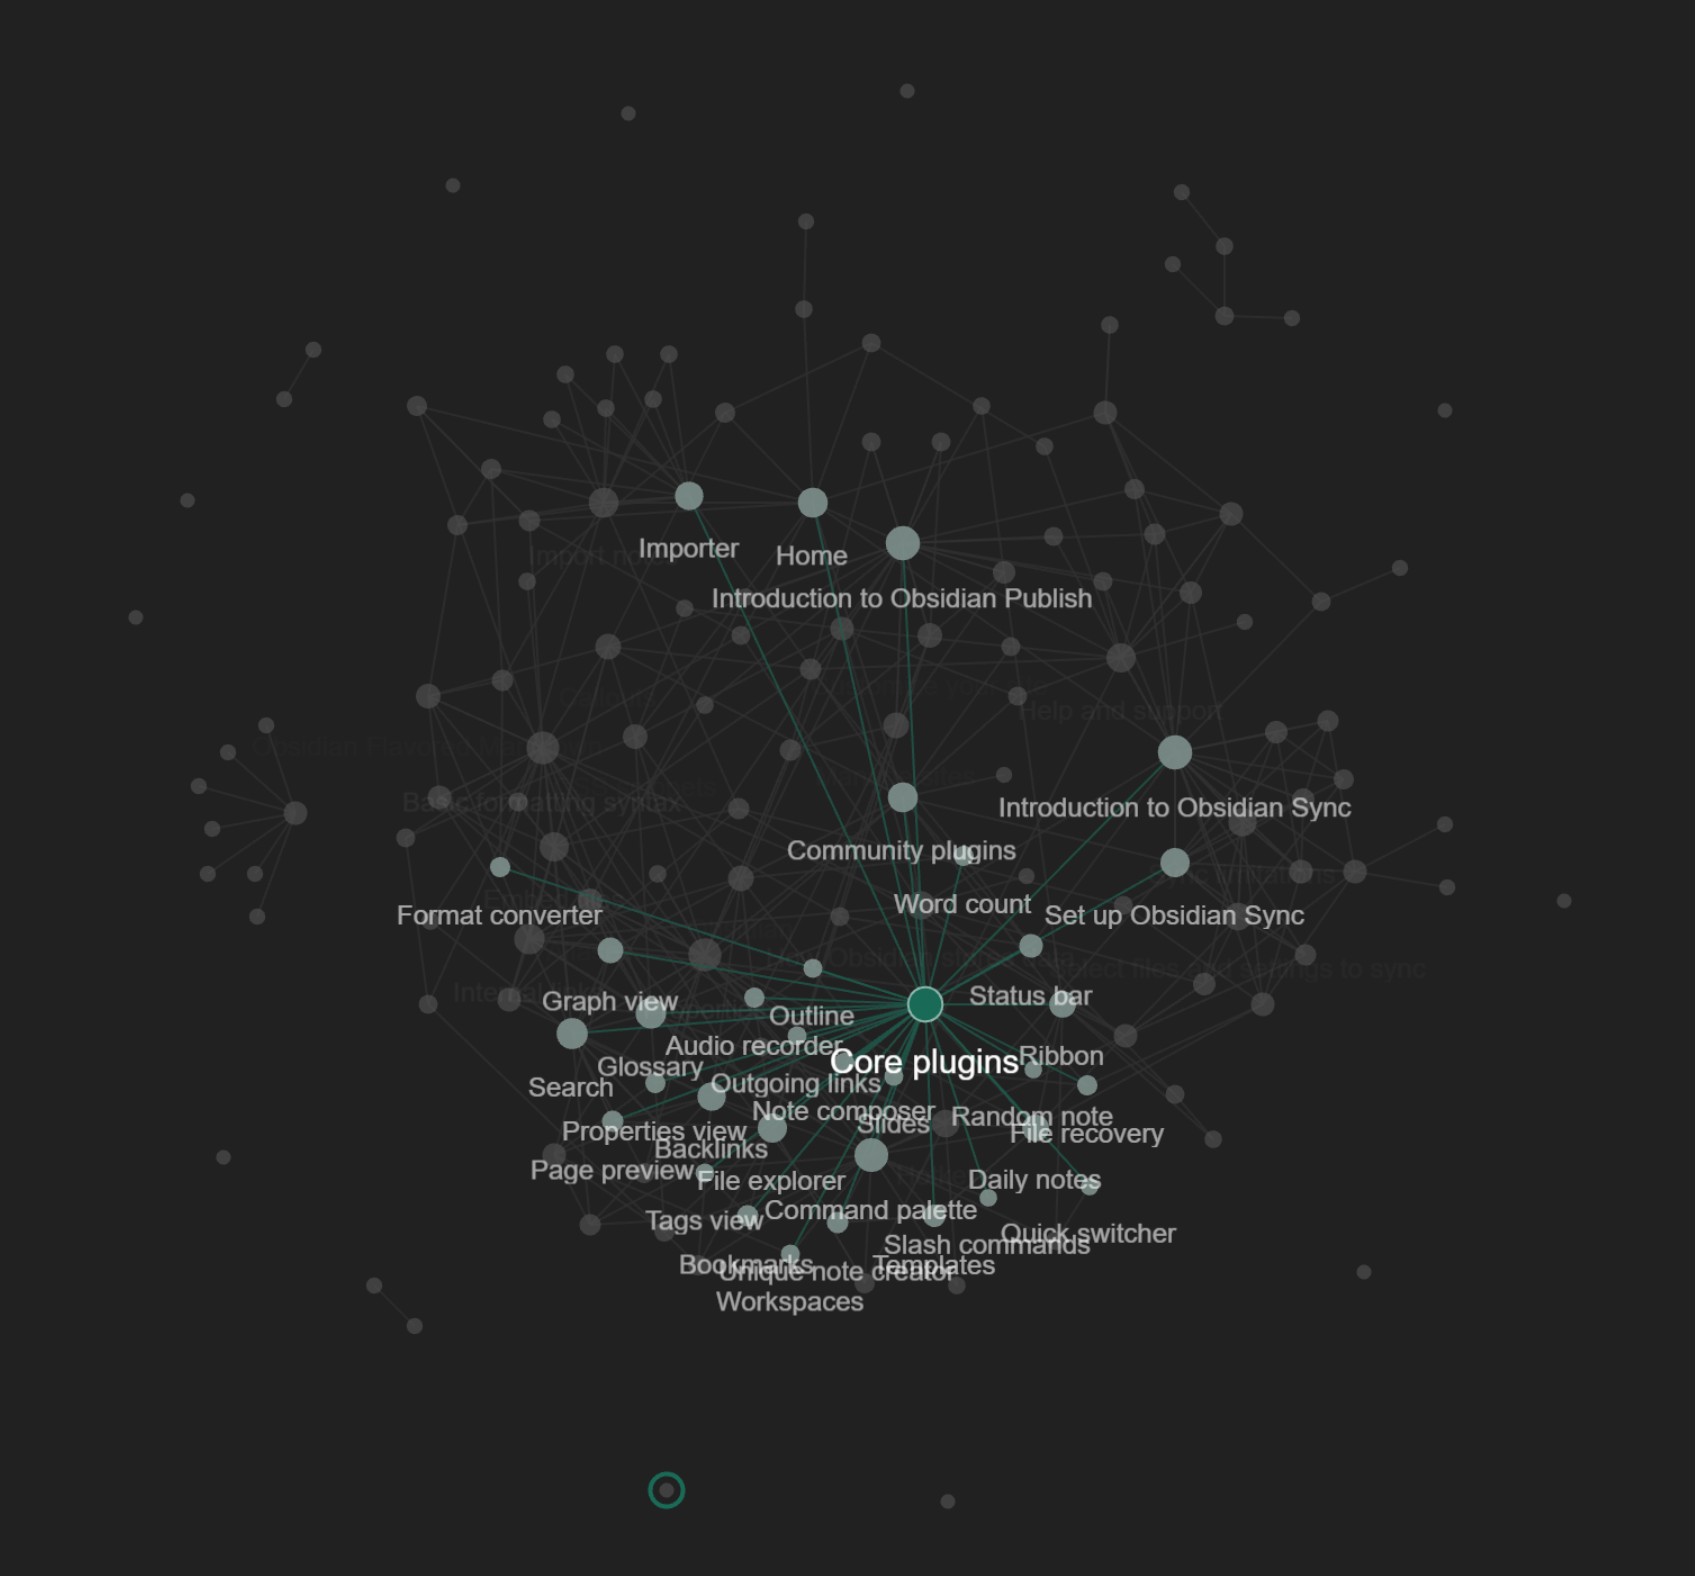
\includegraphics[width=0.8\textwidth]{Research/6_MindMaps/media/Obsidian.png}
    \caption{Obsidian Node Map}
\end{figure}
Obsidian is a notetaking application that uses a node map to visually represent the connections between notes. This is a very powerful tool for visualising the relationships between different pieces of information, however it does not allow for easy searching of specific terms or concepts as it prioritises visual appeal to funcationality.

\subsection*{Integration}
Using the principle of mind maps as a working point I have explored a couple of technical tools i can use to help me achieve my goals. I have found a few frameworks that can help me create a mind map system that is both visually appealing and functional.
\begin{itemize}
    \item D3.js - a powerful JavaScript library for creating data visualisations, it allows for highly customisable and interactive visualisations but requires a lot of coding to set up
    \item Cytoscape.js - a graph theory library that is built on top of D3.js, it provides pre-built components that can be used to create mind maps and other visualisations
    \item Vis.js - a library for creating network visualisations, it is easy to use and provides a lot of functionality out of the box, however it is not as customisable as D3.js or Cytoscape.js
\end{itemize}

While I really like the implementation of mind maps for desktop / larger screen computing. I have identified mobile users to be at disadvantages regarding available screen space for which mind maps are not the most optimal solution. Instead of rethinking my entire viewing system from scratch I have decided to give the user the choice, they can either use a constrained version of the mind map as their searching tool or they can navigate the interface purely using the underlying tag system which drives the main visualisation


